\PassOptionsToPackage{table}{xcolor}
\ifbeamerarticle
  \documentclass[11pt,twoside]{article}
  \usepackage{beamerarticle}
\else
  \documentclass[12pt]{beamer}
\fi
% Packages
\usepackage{mflogo}
\usepackage{tikz}
\usetikzlibrary{fadings,patterns}
\usepackage{pgfplots}
\pgfplotsset{compat=1.8}
\usepgfplotslibrary{statistics}
\usepackage{polyglossia}
\setmainlanguage{english}
\usepackage{tabularx}
\usepackage{booktabs}
\usepackage{placeins}
\usepackage{listings}
\usepackage{dirtree}
%% Bibliography
\usepackage[
  backend=biber,
  style=numeric,
  citestyle=numeric-comp,
  sorting=none
]{biblatex}
\addbibresource{../database.bib}
\ifbeamerarticle
  \let\mycite\cite
\else
  \let\mycite\footfullcite
\fi
%% Fonts
\usepackage{fontspec}
\ifbeamerarticle
  \usepackage{mathpazo}
\else
  \usepackage{cmbright}
\fi
\setmainfont[Ligatures=TeX]{Comenia Serif}
\setsansfont[Ligatures=TeX]{Comenia Sans}
\setmonofont[Scale=MatchLowercase,Ligatures=TeX]{Liberation Mono}
\ifbeamerarticle
  \def\pkg#1{{\sf#1}}
\else
  \let\pkg\emph
\fi
%% Hyperref
\makeatletter
  \@ifpackageloaded{hyperref}{}{\usepackage{hyperref}}
\makeatother
\hypersetup{\ifbeamerarticle color\else hide\fi links,
  linkcolor=black}
% Theming & colors
\usetheme{Antibes}
\usecolortheme{crane}
\usefonttheme{professionalfonts}
\definecolor{green}{RGB}{0,130,0}
\definecolor{yellow}{RGB}{242,212,92}
\definecolor{orange}{RGB}{255,100,0}
% Tabular redefinition
\def\redefinetables{%
  \definecolor{tableOdd}{HTML}{FFF9E5}
  \definecolor{tableEven}{HTML}{FFECB3}
  \definecolor{tableEmph}{HTML}{FFD451}
  \let\oldtabular\tabular
  \let\endoldtabular\endtabular
  \renewenvironment{tabular}%
    {\rowcolors{1}{tableOdd}%
                  {tableEven}%
     \oldtabular}%
    {\endoldtabular}
  \let\oldtabularx\tabularx
  \let\endoldtabularx\endtabularx
  \renewenvironment{tabularx}%
    {\rowcolors{1}{tableOdd}%
                  {tableEven}%
     \oldtabularx}%
     {\endoldtabularx}}
\setlength{\aboverulesep}{0pt}
\setlength{\belowrulesep}{0pt}
\setlength{\extrarowheight}{.75ex}
\def\cellemph{\cellcolor{tableEmph}}
\def\rowemph{\rowcolor{tableEmph}}

% Frametitle for beamer/article redefinition
\ifbeamerarticle
  \let\oldframetitle\frametitle
  \def\frametitle#1{\oldframetitle{#1}\noindent}
\fi

% Miscellanea
\frenchspacing
\ifbeamerarticle\else
  \beamertemplatenavigationsymbolsempty
  \setbeamertemplate{caption}[numbered]
\fi
% Section front page support
\AtBeginSection{\frame{\sectionpage}}
\AtBeginSubsection{\frame{\subsectionpage}}
% Nested itemize fix
% http://tex.stackexchange.com/a/74069/70941
\ifbeamerarticle\else
  \usepackage{etoolbox}
  \setbeamercovered{transparent}
  \makeatletter
  \newcommand*\fix@beamer@close{%
    \ifnum\beamer@trivlistdepth>0%
      \beamer@closeitem%
    \fi}
  \newcommand*\fix@beamer@open{%
    \ifnum\beamer@trivlistdepth>0%
      \gdef\beamer@closeitem{}%
    \fi}
  \BeforeBeginEnvironment{enumerate}{\fix@beamer@close}
  \AfterEndEnvironment{enumerate}{\fix@beamer@open}
  \BeforeBeginEnvironment{itemize}{\fix@beamer@close}
  \AfterEndEnvironment{itemize}{\fix@beamer@open}
  \BeforeBeginEnvironment{description}{\fix@beamer@close}
  \AfterEndEnvironment{description}{\fix@beamer@open}
  \makeatother
\fi
% Metadata
\title{The Form of Theses\\ Written in \LaTeX}
\subtitle{Thesis Presentation}
\date{May 28, 2015}
\author{Vít Novotný}
\institute[FI MU]{Faculty of Informatics,\\Masaryk University in
  Brno}
\begin{document}
\frame{\maketitle}
\frame{\tableofcontents}
\redefinetables
\section{\TeX\ Usage at MU}
\newlength\yearposx
\begin{frame}<1-2>[label=history]
  \frametitle{History of \TeX\ at FI MU}
  \begin{itemize}
    \item<2-> {1994} -- The \textcolor{violet}{ 
      logo} of FI MU
    \item<3-> {1998--2008} -- The
      \textcolor{red}{\pkg{fithesis1}} class
    \item<4-> {2001--2004} -- The
      \textcolor{green}{\pkg{xslt2}} module
    \item<5-> {2008--2015} -- The
      \textcolor{blue}{\pkg{fithesis2}} class
    \item<6-> {2013} -- The
      \textcolor{orange}{\pkg{comenia}} package
  \end{itemize}\medskip
  \begin{tikzpicture}[scale=\ifbeamerarticle0.57\else0.46\fi]
    \foreach \x in {1994,1998,2001,2004,2008,2013,2015}{
      \pgfmathsetlength\yearposx{(\x-1994)*1cm};
      \coordinate (y\x) at (\yearposx,0);
      \coordinate (y\x t) at (\yearposx,0.75mm);
      \draw (\yearposx,+3pt) -- (\yearposx,-3pt);}
    \draw [->] (y1994) -- (y2015);
    \uncover<2-> {\node at (y1994) [above=3pt]
      {{1994}};}
    \only<2-> {\fill[violet] (y1994) circle (5pt);}
    \uncover<3-> {
      \node at (y1998) [below=3pt] {{1998}};
      \node at (y2008) [above=3pt] {{2008}};}
    \only<3-> {
      \draw[red,line width=0.75mm] (y1998) -- (y2008);
      \fill[red] (y1998) circle (5pt);
      \fill[red] (y2008) circle (5pt);}
    \uncover<4-> {
      \node at (y2001) [above=3pt] {{2001}};
      \node at (y2004) [below=3pt] {{2004}};}
    \only<4-> {
      \draw[green,line width=0.75mm] (y2001t) -- (y2004t);
      \fill[green] (y2001t) circle (5pt);
      \fill[green] (y2004t) circle (5pt);}
    \uncover<5-> {
      \node at (y2015) [below=3pt] {{2015}};}
    \only<5-> {
      \draw[blue,line width=0.75mm] (y2008) -- (y2015);
      \fill[blue] (y2008) circle (5pt);
      \fill[blue] (y2015) circle (5pt);}
    \uncover<6-> {\node at (y2013) [above=3pt]
      {{2013}};}
    \only<6-> {\fill[orange] (y2013t) circle (5pt);}
  \end{tikzpicture}
\end{frame}
\begin{frame}
  \begin{figure}
    \centering
    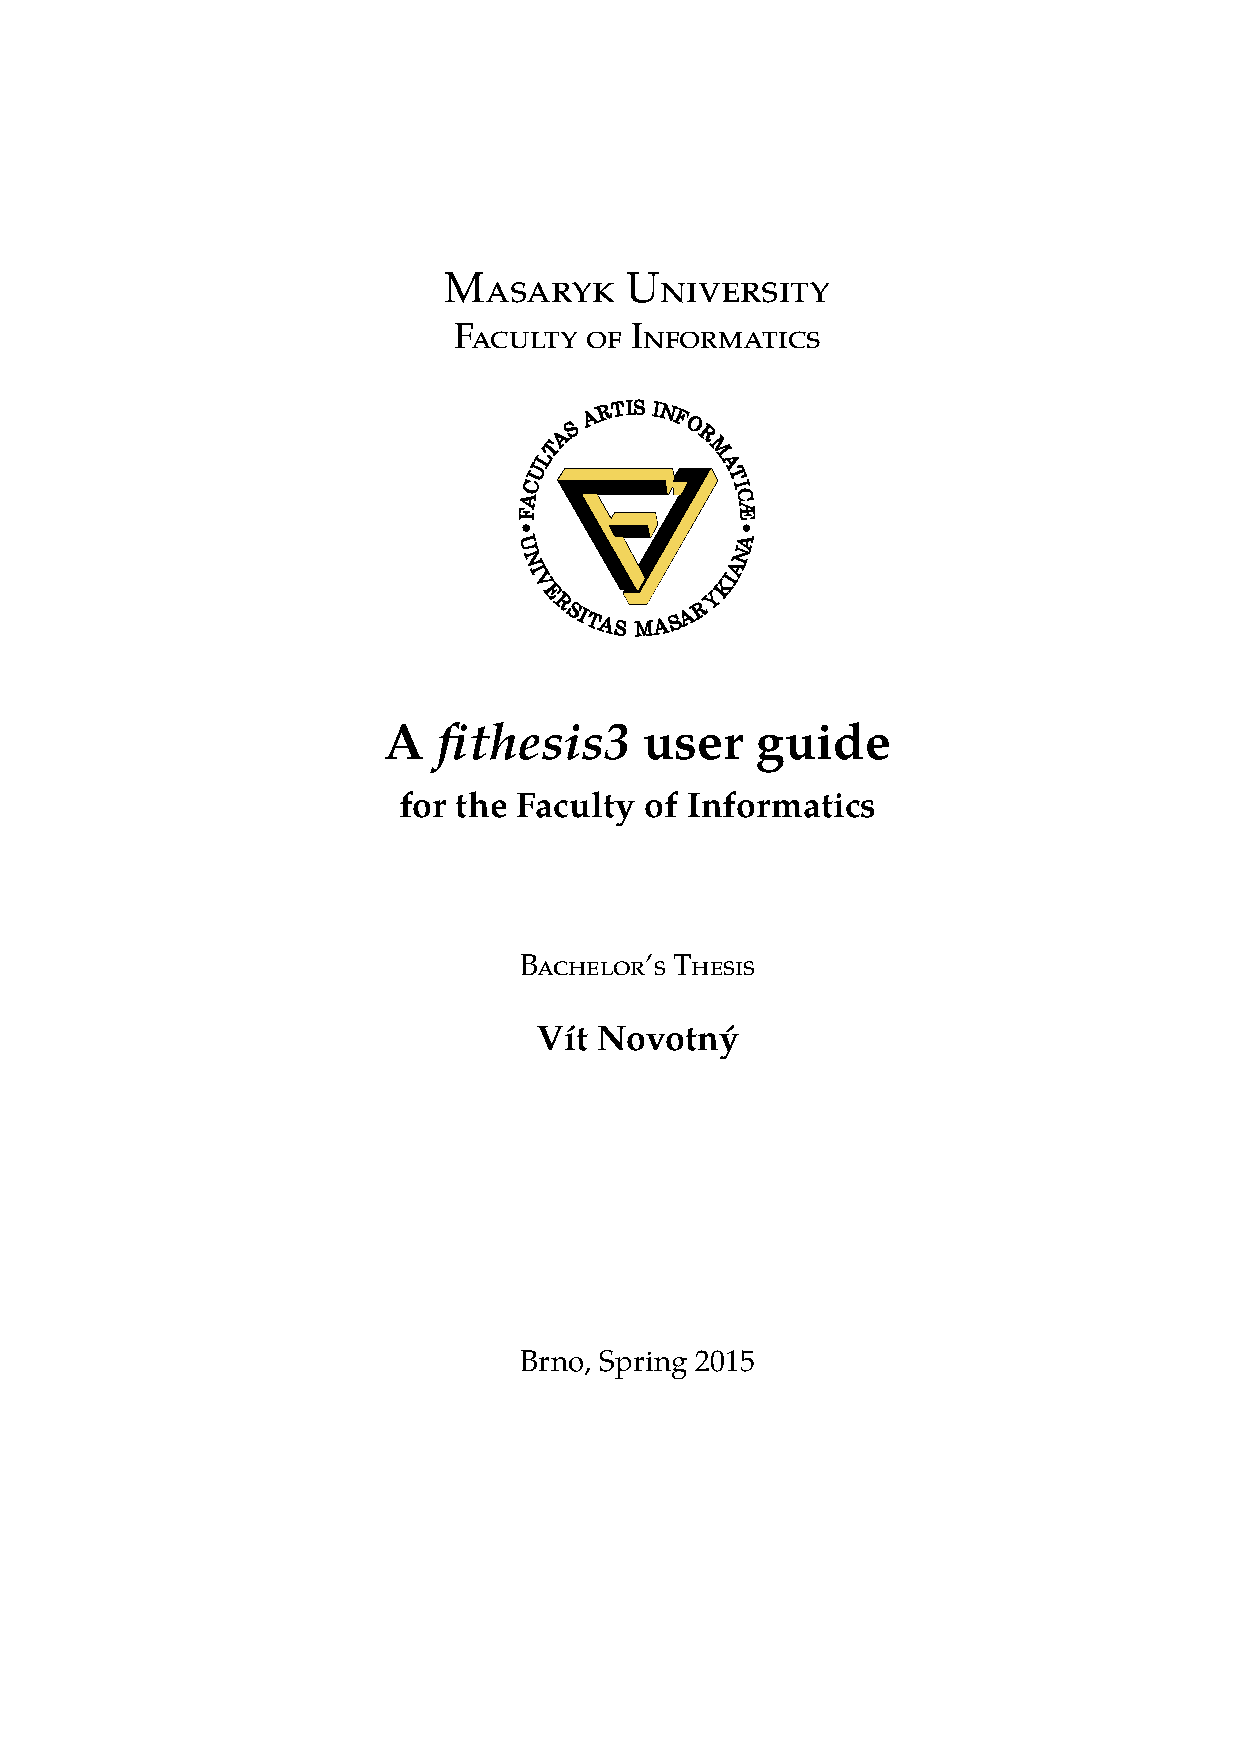
\includegraphics[width=\ifbeamerarticle4\else5\fi cm]
      {../fithesis3/fithesis3/logo/mu/color/fi}
    \caption{The logo of FI MU designed by Doc. Petr Sojka and
      implemented\ifbeamerarticle~\cite{zlatuska95}\else%
      \footnotemark[1]\fi\ by the founding Dean of FI, Prof. Jiří
      Zlatuška}
    \ifbeamerarticle\else
      \footnotetext[1]{\fullcite{zlatuska95}}
    \fi
  \end{figure}
\end{frame}
\againframe<2->{history}
\subsection{User Survey}
\begin{frame}[c]
  \begin{table}[!b]
    \begin{tabularx}{\textwidth}{Xcr}
      \textbf{On which faculty of
      MU do you study?} & \textbf{\#}
      \\ \toprule Faculty of Informatics          & $82$
      \\ Faculty of Science                       &  $3$
      \\ Faculty of Education                     &  $2$
      \\ Faculty of Social Studies                &  $2$
      \\ Faculty of Law                           &  $1$
      \\ Faculty of Medicine                      &  $1$
      \\ Faculty of Arts                          &  $1$
      \\ Faculty of Economics and Administration  &  $1$
      \\ Faculty of Sports Studies                &  $0$
      \\
    \end{tabularx}
    \caption{The distribution of the questionnaire
      respondents across the faculties of MU}
  \end{table}
\end{frame}
\begin{frame}[c]
  \begin{table}[!b]
    \begin{tabularx}{\textwidth}{Xcr}
      \textbf{Which academic degree are you pursuing?} &
      \textbf{\#} \\
      \toprule
      Bachelor's degree  & $70$ \\
      Master's degree    & $17$ \\
      Doctorate          & $2$  \\
      \bottomrule
      \textbf{Total}     & $\mathbf{89}$
    \end{tabularx}
    \caption{The highest academic degrees currently pursued by the
      respondents of the questionnaire}
  \end{table}
\end{frame}
\begin{frame}
  \begin{table}[!b]
    \begin{tabularx}{\textwidth}{Xcr}
      \textbf{Which application do you use / are you planning to
      use to write your thesis?} & \textbf{\#} \\
      \toprule
      \TeX\ / \LaTeX          & $65$          \\
      Microsoft Office        & $16$          \\
      Apache OpenOffice, LibreOffice or another free office
      software suite          & $4$           \\
      Other                   & $4$           \\
      Google Documents        & $0$           \\
      \bottomrule
      \textbf{Total}          & $\mathbf{89}$ 
    \end{tabularx}
    \caption{The software the respondents of the questionnaire
      were using or planning to use to write their theses}
  \end{table}
\end{frame}
\begin{frame}
  \begin{table}[!b]
    \begin{tabularx}{\textwidth}{Xcr}
      \textbf{Are you planning to use the \pkg{fithesis1}
        class?} & \textbf{\#} \\
      \toprule    Yes                       & $47$
      \\ Maybe, I did not know it existed   & $10$
      \\ No, I'm going to use another class & $5$
      \\ Other                              & $2$
      \\ No, I'm going to use plain \TeX{}  & $1$
      \\ \bottomrule
      \textbf{Total}  & $\mathbf{65}$ 
    \end{tabularx}
      \caption{The attitude towards the usage of the \pkg{fithesis1}
      class amongst those respondents who claimed to be using or
      planning to use \TeX{} to typeset their theses}
  \end{table}
\end{frame}
\begin{frame}
  \frametitle{Conclusion}
  The majority of respondents:
  \begin{itemize}
    \item were FI bachelor's degree students,
    \item preferred \pkg{fithesis1} over the alternatives.
  \end{itemize}
\end{frame}\FloatBarrier
\subsection{Analysis of Existing Theses}
\begin{frame}
  \begin{table}[!b]
    \scalebox{\ifbeamerarticle1\else0.9\fi}{\begin{tabularx}%
      {\ifbeamerarticle1\else1.11\fi\textwidth}{Xrr}
      \textbf{Faculty} & \textbf{\#} & \textbf{\%} \\
      \toprule
      Faculty of Arts                         & $10\,000$ & $21.98$ \\% 1421
      Faculty of Education                    & $8\,219$  & $18.07$ \\% 1441
      Faculty of Social Studies               & $5\,599$  & $12.31$ \\% 1423
      Faculty of Science                      & $5\,275$  & $11.60$ \\% 1431
      Faculty of Law                          & $4\,824$  & $10.60$ \\% 1422
      Faculty of Economics and Administration & $4\,591$  & $10.09$ \\% 1456
      Faculty of Informatics                  & $2\,904$  &  $6.38$ \\% 1433
      Faculty of Medicine                     & $2\,014$  &  $4.43$ \\% 1411
      Faculty of Sports Studies               & $2\,062$  &  $4.53$ \\% 1451
      \bottomrule
      \textbf{Total}     & $\mathbf{45\,488}$ & $\mathbf{100.00}$
    \end{tabularx}}
    \caption{The distribution of theses defended between 2010--2015
      across the faculties of MU}
  \end{table}
\end{frame}
\begin{frame}
  \begin{table}[!b]
    \begin{tabularx}{\textwidth}{Xrr}
      \textbf{Degree} & \textbf{\#} & \textbf{\%} \\
      \toprule
      Bachelor's & $22\,288$ & $49.00$ \\
      Master's   & $20\,761$ & $45.64$ \\
      Doctoral   &  $2\,231$ &  $4.90$ \\
      Lifelong   &     $208$ &  $0.46$ \\
      \bottomrule
      \textbf{Total} & $\mathbf{45\,488}$ & $\mathbf{100.00}$
    \end{tabularx}
    \caption{The distribution of theses defended between 2010--2015
      across the study programme degrees}
  \end{table}
\end{frame}\begin{frame}
  A thesis was considered to be written using \TeX, if one
  or more files submitted with it satisfied one or more of the
  following conditions: \begin{itemize}
    \item The suffix was \texttt{tex}.
    \item The magic number was that of a DVI file.
    \item The MIME type was \texttt{application/postscript} and
      the file contained the \texttt{TeXDict} substring suggesting
      that the file was a PS document, which had been created
      using the \textsf{dvips} utility.
    \item The MIME type was \texttt{application/pdf} and either
      the \texttt{Creator} or the \texttt{Producer} PDF 
      header contained the \texttt{TeX} substring suggesting that
      the file had been created using either the \textsf{dvipdfm}
      utility or a \TeX\ engine, which supports PDF output.
  \end{itemize}
\end{frame}
\begin{frame}
  \begin{table}[!b]
    \scalebox{\ifbeamerarticle1\else0.83\fi}{\begin{tabularx}%
      {\ifbeamerarticle1\else1.2\fi\textwidth}{Xrrr}
      \textbf{Faculty} & \textbf{With \TeX} & \textbf{Total} &
      \textbf{\%} \\
      \toprule
      Faculty of Informatics       & $1\,716$ & $2\,904$  &
      $59.09$ \\% 1433
      Faculty of Science           & $786$     & $5\,275$  &
      $14.90$ \\% 1431
      Faculty of Economics and Administration & $64$ & $4\,591$ &
      $1.39$  \\% 1456
      Faculty of Arts              & $69$      & $10\,000$ &
      $0.69$  \\% 1421
      Faculty of Medicine          & $8$       & $2\,014$  &
      $0.40$  \\% 1411
      Faculty of Law               & $15$      & $4\,824$  &
      $0.31$  \\% 1422
      Faculty of Education         & $19$      & $8\,219$  &
      $0.23$  \\% 1441
      Faculty of Social Studies    & $12$      & $5\,599$  &
      $0.21$  \\% 1423
      Faculty of Sports Studies    & $3$       & $2\,062$  &
      $0.15$  \\% 1451
      \bottomrule
      \textbf{Total} & $\mathbf{2\,692}$ & $\mathbf{45\,488}$ &
      $\mathbf{5.92}$
    \end{tabularx}}
    \caption{The distribution of theses written using \TeX,
      which were defended during 2010--2015 across the faculties of
      MU}
  \end{table}
\end{frame}
\begin{frame}
  \begin{table}[!b]
    \scalebox{\ifbeamerarticle1\else0.85\fi}{\begin{tabularx}%
      {\ifbeamerarticle1\else1.17\fi\textwidth}{Xlrrrrrr}
      \textbf{Degree} & \textbf{Fac.} & \textbf{2010} &
      \textbf{2011} & \textbf{2012} & \textbf{2013} & \textbf{2014}
      & $R$\\
      \toprule
      \ifbeamerarticle
        Bachelor's
          & FI  & $58.92$ & $59.44$ & $49.54$ & $53.77$ &
            $59.06$ & \textcolor{red}{$-0.195$} \\
          & Sci & $11.55$ & $13.00$ & $15.90$ & $19.79$ &
            $15.16$ & \textcolor{green}{$+0.703$} \\
          & All & $5.08$ & $6.19$ &
            $6.00$ & $6.08$ & $6.24$ &
            \textcolor{green}{$+0.731$} \\ \midrule
        Master's
          & FI  & $60.61$ & $59.91$ & $60.08$ & $64.50$ &
            $57.96$ & \textcolor{red}{$-0.046$} \\
          & Sci & $19.38$ & $13.54$ & $13.75$ & $13.78$ &
            $17.71$ & \textcolor{red}{$-0.180$} \\
          & All & $6.02$ & $4.88$ &
            $5.22$ & $6.59$ & $6.29$ &
            \textcolor{green}{$+0.490$} \\ \midrule
      \else
        Bachelor's &&&& \multicolumn{1}{c}{\vdots} &&& \\ \midrule
        Master's   &&&& \multicolumn{1}{c}{\vdots} &&& \\ \midrule
      \fi
      Doctoral
        & FI  & $100.00$ & $76.67$ & $71.88$ & $83.87$ &
          $90.91$ & \textcolor{red}{$-0.155$} \\
        & Sci & $18.09$ & $10.71$ & $12.75$ & $10.19$ &
          $8.85$ & \only<2>{\cellemph}\textcolor{red}{$-0.830$} \\
        & All & $8.83$ & $8.23$ &
          $8.41$ & $9.38$ & $7.43$ &
          \textcolor{red}{$-0.361$} \\
        \bottomrule
      \textbf{All}
        & \textbf{FI} & $\mathbf{60.83}$ &
          $\mathbf{60.53}$ & $\mathbf{54.92}$ & $\mathbf{60.57}$ &
          $\mathbf{59.34}$ & \textcolor{red}{$\mathbf{-0.188}$} \\
        & \textbf{Sci} & $\mathbf{14.86}$ &
          $\mathbf{12.96}$ & $\mathbf{14.74}$ & $\mathbf{16.55}$ &
          $\mathbf{15.45}$ &
          \textcolor{green}{$\mathbf{+0.577}$}\\
        & \textbf{All} & $\mathbf{5.67}$ &
          $\mathbf{5.70}$ & $\mathbf{5.73}$ &
          $\mathbf{6.41}$ & $\mathbf{6.28}$ &
          \only<2>{\cellemph}\textcolor{green}{$\mathbf{+0.855}$}
      \end{tabularx}}
    \begin{overlayarea}{\textwidth}{8em}
    \only<1>{\caption{The percentage of theses written using \TeX\ 
      which were defended in each year during 2010--2014 and the
      sample correlation coefficient $R$ between the percentage and
      the years with remarkably strong correlations emphasized}}
    \ifbeamerarticle\else\addtocounter{table}{1}\fi
    \only<2>{\smallskip\footnotesize There was a marked and steady
      increase in the use of \TeX\ for the typesetting of theses
      during 2010--2014. This does not necessarily hold true for
      individual faculties and degree study programmes, as
      exemplified by the pronounced downwards trend in the use of
      \TeX\ for the typesetting of doctoral theses at Sci.}
    \end{overlayarea}
  \end{table}
\end{frame}
\begin{frame}
  \begin{table}[!b]
    \scalebox{\ifbeamerarticle1\else0.9\fi}{\begin{tabularx}%
      {\ifbeamerarticle1\else1.11\fi\textwidth}{Xrrrrr}
      &\textbf{Without \TeX}&E(\textbf{With \TeX})
      &O(\textbf{With \TeX})&$(\text{E}-\text{O})^2/\text{E}$
      \\ \toprule
      \textbf{\parbox[t]{1em}{\centering A}} 
        &$15\,476$&$987.635$&\only<3>{\cellemph}
        \textcolor{green}{$1\,181$}&
        \only<3>{\cellemph}$37.858$\\
      \textbf{\parbox[t]{1em}{\centering B}}
        &$9999$&$638.108$&\textcolor{red}{$587$}&$4.093$\\
      \textbf{\parbox[t]{1em}{\centering C}}
        &$7\,926$&$505.815$&\only<3>{\cellemph}
        \textcolor{red}{$381$}&
        \only<3>{\cellemph}$30.799$\\
      \textbf{\parbox[t]{1em}{\centering D}}
        &$4\,020$&$256.545$&\only<3>{\cellemph}
        \textcolor{red}{$194$}&
        \only<3>{\cellemph}$15.248$\\
      \textbf{\parbox[t]{1em}{\centering E}}
        &$2\,783$&$177.603$&\textcolor{red}{$128$}&$13.853$\\
      \textbf{\parbox[t]{1em}{\centering F}}
        &$1\,979$&$126.294$&\textcolor{green}{$145$}&
        $2.771$\\
      \bottomrule
      \textbf{Total} &$\mathbf{42\,183}$&$\mathbf{2\,692}$&
        $\mathbf{2\,692}$&$\only<2>{\cellemph}\mathbf{104.623}$
    \end{tabularx}}
    \begin{overlayarea}{\textwidth}{8em}
      \only<1>{\caption{The contingency table of the
        numbers of marks awarded to theses written and defended
        during 2010--2015 with Pearson's goodness-of-fit measure
        $(\text{E}-\text{O})^2/\text{E}$ between the expected (O) and
        the observed (E) numbers of marks awarded to theses written
        using \TeX}}
      \iffalse\else
      \only<2>{\smallskip\footnotesize There was an overwhelming difference
        in the distribution of grades given to theses written using
        and not using \TeX:\begin{equation}\nonumber
        \sum_{\text{A},\text{B},\ldots,\text{F}}
        (\text{E}-\text{O})^2/\text{E}=104.623\gg11.07=
        \chi_{0.95}^2(5)
      \end{equation}}
      \only<3>{\smallskip\footnotesize Theses written using \TeX\
        had been awarded:
        \begin{itemize}
          \item grade A statistically significantly
            \textcolor{green}{more often},
          \item grades C and D statistically significantly
            \textcolor{red}{less often}.
        \end{itemize}
      }\fi
    \end{overlayarea}
  \end{table}
\end{frame}
\begin{frame}
  \begin{figure}
    \centering
    \ifbeamerarticle\else\scalebox{0.95}{\fi%
    \begin{tikzpicture}
      \begin{axis}
        [
          ytick={1,2,3,4,5,6},
          xticklabels={,,A,B,C,D,E,F},
          yticklabels={With \TeX{} (at Sci),
                       Without \TeX{} (at Sci),
                       With \TeX{},
                       Without \TeX{},
                       With \TeX{} (at FI),
                       Without \TeX{} (at FI)},
        ]
        \addplot+[
          boxplot prepared={
            lower quartile=1,
            median=1,
            upper quartile=2,
            upper whisker=3,
            lower whisker=1,
            % average=1.9148387097
          },
        ] table[row sep=\\,y index=0] {
          data\\ 4\\ 5\\ 6\\
        };
        \addplot+[
          boxplot prepared={
            lower quartile=1,
            median=2,
            upper quartile=3,
            upper whisker=6,
            lower whisker=1,
            % average=2.0201768307
          },
        ] table[row sep=\\,y index=0] {
          data\\
        };
        \addplot+[
          boxplot prepared={
            lower whisker=1,
            lower quartile=1,
            median=2,
            upper quartile=3,
            upper whisker=6,
            % average=2.2110091743
          },
        ] table[row sep=\\,y index=0] {
          data\\
        };
        \addplot+[
          boxplot prepared={
            lower whisker=1,
            lower quartile=1,
            median=2,
            upper quartile=3,
            upper whisker=6,
            % average=2.3971979233
          },
        ] table[row sep=\\,y index=0] {
          data\\
        };
        \addplot+[
          boxplot prepared={
            lower whisker=1,
            lower quartile=1,
            median=2,
            upper quartile=3,
            upper whisker=6,
            % average=2.3565375303
          },
        ] table[row sep=\\,y index=0] {
          data\\
        };
        \addplot+[
          boxplot prepared={
            lower whisker=1,
            lower quartile=2,
            median=3,
            upper quartile=5,
            upper whisker=6,
            % average=3.1209262436
          },
        ] table[row sep=\\,y index=0] {
          data\\
        };
      \end{axis}
    \end{tikzpicture}
    \ifbeamerarticle\else}\fi%
    \caption{A box plot of the grades of theses written and
      defended during 2010--2015 at FI, Sci and all the
      faculties of MU}
  \end{figure}
\end{frame}
\begin{frame}
  \frametitle{Conclusion}
  During 2010--2014, the usage of \TeX\ for the typesetting of
  theses at MU: \begin{itemize}
    \item increased by $0.61\%$ across all faculties,
    \item correlated with significantly better grades.
  \end{itemize}
\end{frame}
\FloatBarrier
\section{Review of Existing Templates}
\def\right#1{{\hfill\ifbeamerarticle\else
    \textcolor{white!33!black}{\scriptsize
  \fi(#1)\ifbeamerarticle\else}\fi}}
\begin{frame}[fragile]
  \frametitle{Templates of Czech Universities}
  The templates of the following universities were reviewed:
  \begin{enumerate}
    \item Charles University\right{\pkg{CUStyle}, official template}
    \item Czech Technical University\right{\pkg{CTUStyle, felthesis}}
    \item Mendel University in Brno\right{\texttt{dipp.sty}}
    \item Brno University of Technology\right{\texttt{thesis.sty}}
    \item Technical University of Liberec\right{\pkg{tul+tulthesis}}
    \item Technical University of Ostrava\right{\pkg{diploma}}
    \item Palacký University in Olomouc\right{\pkg{KIDiplom},
      \texttt{maam-dipl.sty}}
    \item Masaryk University in Brno\right{\texttt{sci.muni.thesis.sty}}
  \end{enumerate}
\end{frame}
\begin{frame}<1-3>[label=conclusion]
  \frametitle{Conclusion from the Review}
  \uncover<1,2,4->{Features to consider:}\begin{itemize}
%   \item<1,4,5,10> Separation of concerns
%     \right{\pkg{tul+tulthesis, KIDiplom}}
    \item<1,4,5> Moderate use of color \right{\pkg{CTUStyle, CUStyle,
      tul}}
    \item<1,4,6> Unicode \TeX\ engine support\right{\pkg{tul+tulthesis},
      \texttt{dipp.sty}}
    \item<1,4,7> PDF metadata stamping \right{\pkg{felthesis}}
    \item<1,4,8,9> Support for various
      faculties\right{\pkg{tul+tulthesis}}
    \item<2> Additional mark-up
      \right{\texttt{dipp.sty}, \texttt{thesis.sty}, \pkg{diploma}}
    \item<2> Homebrew \textsc{Bib}\LaTeX\ ISO-690 citation styles
      \right{\pkg{KIdiplom}}
  \end{itemize}\uncover<3,4>{Problems to avoid:}\begin{itemize}
    \item<3,4> Lack of double-sided typesetting\right{\pkg{KIdiplom}}
    \item<3,4> Overly large \texttt{\string\textwidth}\right{All except
      \pkg{tul+tulthesis, felthesis}}
  \end{itemize}
\end{frame}
\section{Design and Implementation}
\againframe<4,5>{conclusion}
{\def\showlogo#1{%
  \includegraphics[width=2cm]{%
    ../fithesis3/fithesis3/logo/mu/color/#1}}
\def\logokern{\kern 1ex}
\begin{frame}
  \begin{figure}[!]
    \centering
    \showlogo{base}\logokern%
    \showlogo{fsps}\logokern%
    \showlogo{phil}\logokern%
    \showlogo{law}\logokern%
    \showlogo{sci}\\<all>[1ex]%
    \showlogo{fss}\logokern%
    \showlogo{econ}\logokern%
    \showlogo{med}\logokern%
    \showlogo{ped}\logokern%
    \showlogo{fi}%
    \caption{The colorful logos of MU}
  \end{figure}
\end{frame}}
\begin{frame}
  \begin{figure}[!]
    \centering
    \begin{tabularx}{\textwidth}{lll>{\raggedright\arraybackslash}X}
    \toprule
    Day & Min Temp & Max Temp & Summary \\ \midrule
    Monday & $11^{\circ}\mathrm{C}$ & $22^\circ\mathrm{C}$ &
      A clear day with lots of sunshine.\\
    Tuesday & $9^{\circ}\mathrm{C}$ & $19^\circ\mathrm{C}$ &
      Cloudy with rain, across many northern regions.\\
    Wednesday & $10^{\circ}\mathrm{C}$ & $21^\circ\mathrm{C}$ &
      Rain will still linger for the morning.\\
    \bottomrule
    \end{tabularx}
    \caption{Other colorful typographic elements}
  \end{figure}
\end{frame}
\againframe<5-8>{conclusion}
\lstset{
  backgroundcolor=\color{white}, 
  basicstyle=\ifbeamerarticle\footnotesize\else\scriptsize\fi%
    \ttfamily,
  breakatwhitespace=false,        
  breaklines=true,                 
  captionpos=n,                    
  commentstyle=\color{green},   
  escapeinside={\%*}{*)},        
  extendedchars=true,              
  keywordstyle=\color{blue},       
  language=[LaTeX]TeX,            
  escapeinside={\%*}{*)},    
  showspaces=false,               
  showstringspaces=false,          
  showtabs=false,                  
  stringstyle=\color{violet},   
  tabsize=2,                      
  title=\lstname,                  
  morekeywords={not,\},\{,preconditions,effects },            
  deletekeywords={time}}
\begin{frame}[fragile]
  \begin{figure}[!]
    \begingroup
    \lstset{basicstyle=\ifbeamerarticle\scriptsize\else\tiny\fi%
      \ttfamily}
    \begin{lstlisting}
\documentclass[12pt]{fithesis2}
\usepackage[english]{babel}       % Multilingual support
\usepackage[utf8]{inputenc}       % UTF-8 encoding
\usepackage[T1]{fontenc}          % T1 font encoding
\thesislang{en}                   % The language of the thesis
\thesistitle{Sample Thesis}       % The title of the thesis
\thesissubtitle{Bachelor Thesis}  % The type of the thesis
\thesisstudent{Jane Doe}          % Your name
\thesiswoman{true}                % Your gender
\thesisfaculty{fi}                % Your faculty
\thesisyear{Spring \the\year}     % The academic term
\thesisadvisor{John Foo, Ph.D.}   % Your advisor
\begin{document}
  \FrontMatter                    % The front matter
    \ThesisTitlePage                % The title page
    \begin{ThesisDeclaration}
      \DeclarationText\AdvisorName\end{ThesisDeclaration}
    \begin{ThesisThanks}I would like to thank\,\dots\end{ThesisThanks}
    \begin{ThesisAbstract}The aim of the\,\dots\end{ThesisAbstract}
    \begin{ThesisKeyWords}keyword1, keyword2\,\dots\end{ThesisKeyWords}
    \tableofcontents                % The table of contents
  \MainMatter                     % The main matter
  % Here goes the text of the thesis
\end{document}
    \end{lstlisting}
    \endgroup
    \caption{A minimal \pkg{fithesis2} document}
  \end{figure}
\end{frame}
\begin{frame}[fragile]
  \begin{figure}[!]
    \begin{lstlisting}
\documentclass{fithesis3}
\usepackage[english]{babel}
\thesissetup{faculty = sci}
\begin{document}
  % Here goes the text of the thesis
\end{document}
    \end{lstlisting}
    \caption{A minimal \pkg{fithesis3} document}
  \end{figure}
\end{frame}
\begin{frame}[fragile]
  \begin{figure}[!]
    \begin{lstlisting}
\documentclass[twoside,color]{fithesis3}
\usepackage[english]{babel}
\thesissetup{
  title       = The Form of Theses Written in LaTeX,
  TeXtitle    = The Form of Theses\\ Written in \LaTeX,
  author      = Vít Novotný,
  advisor     = {Doc. RNDr. Petr Sojka, Ph.D.},
  keywords    = {latex document classes, thesis typesetting,
    fithesis, tex usage statistics},
  TeXkeywords = {\LaTeX\ document classes, thesis typesetting,
    \textsf{fithesis}, \TeX\ usage statistics},
  assignment  = {./misc/declaration.pdf, 1, {},
                 ./misc/assignment.pdf,  1, {}}}
\thesislong{abstract}{This bachelor's thesis aims to assess
  existing templates for the typesetting of theses and ...}
\thesislong{thanks}{I wish to express my most sincere gratitude
  and appreciation to Doc. RNDr. Petr Sojka for sharing ...}
\begin{document}
  % Here goes the text of the thesis
\end{document}
    \end{lstlisting}
    \caption{A standard \pkg{fithesis3} document}
  \end{figure}
\end{frame}
\begin{frame}<1>[label=design]
  \frametitle{Design}
  \begin{itemize}
    \item<1->\pkg{Fithesis1} and \pkg{2} mix logic, locales and
      presentation.
    \item<2-> Proper support for faculties requires the addition of:
      \begin{itemize}
        \item<2-> per-faculty document layout definitions,
        \item<3-> per-faculty locale strings,
        \item<4-> per-faculty presentation code.
      \end{itemize}
    \item<5-> Non-functional requirements:
      \begin{itemize}
        \item<5-> Adherence to the open/closed principle
        \item<6-> Extensive documentation
      \end{itemize}
  \end{itemize}
\end{frame}
\begin{frame}[fragile]
  \begin{figure}[!]
    \begin{lstlisting}
\def\thesistitle#1{\gdef\@thesistitle{#1}}
\def\thesissubtitle#1{\gdef\@thesissubtitle{#1}}
\def\thesisstudent#1{\gdef\@thesisstudent{#1}}
\newif\ifwoman\womanfalse
\def\thesiswoman#1{\def\@thesiswoman{#1}
  \ifx\@thesiswoman\True\womantrue\else\womanfalse\fi}
\def\@w{\ifwoman a\else\fi} 
    \end{lstlisting}
    \caption{The input processing code within \pkg{fithesis1}
      and \pkg{2}}
  \end{figure}
\end{frame}
\begin{frame}[fragile]
  \begin{figure}[!]
    \begin{lstlisting}
\def\AbstractTitlecs{Shrnutí}
\def\AbstractTitlesk{Zhrnutie}
\def\AbstractTitleen{Abstract}
\def\DeclarationTextcs{%
  %*Prohlašuji*), že tato \expandafter\lowercasewrapper%
  \@thesissubtitle\ je mým %*původním*) autorským dílem,
  které jsem vypracoval\@w\ %*samostatně*). %*Všechny*)
  zdroje, prameny a literaturu, které jsem %*při*)
  vypracování %*používal*)\@w\ nebo z~nich čerpal\@w,
  v~práci %*řádně*) cituji s~uvedením úplného odkazu na
  %*příslušný*) zdroj.}
    \end{lstlisting}
    \caption{The locale strings within \pkg{fithesis1} and
      \pkg{2}}
  \end{figure}
\end{frame}
\begin{frame}[fragile]
  \begin{figure}[!]
    \begin{lstlisting}
\renewcommand*\l@chapter{%
  \@dottedtocline{1}{0em}{1.5em}}
\renewcommand*\l@section{%
  \@dottedtocline{2}{1.5em}{2.3em}}
\renewcommand*\l@subsection{%
  \@dottedtocline{3}{3.8em}{3.2em}}
\renewcommand*\l@subsubsection{%
  \@dottedtocline{4}{7.0em}{3.8em}}
    \end{lstlisting}
    \caption{The presenation code within \pkg{fithesis1} and
      \pkg{2}}
  \end{figure}
\end{frame}
\againframe<2-4>{design}
\begin{frame}[fragile]
  \begin{figure}[!]
    \begin{lstlisting}
\if\@thesisfaculty\Fi
  \def\@mainMatter{%
    % ...
  \def\@titlePage{%
    % ...
  % ...
\else\if\@thesisfaculty\Sci
  % ...
% ...
\fi\fi\fi\fi\fi\fi\fi\fi\fi
    \end{lstlisting}
    \caption{A simple extension of \pkg{fithesis1} and \pkg{2}
      to add support for per-faculty document layouts}
  \end{figure}
\end{frame}
\begin{frame}[fragile]
  \begin{figure}[!]
    \begin{lstlisting}
\if\@thesisfaculty\Fi
  \def\DeclarationTextcs{%
    %*Prohlašuji*), že tato \expandafter\lowercasewrapper%
    \@thesissubtitle\ je mým %*původním*) autorským dílem,
    které jsem vypracoval\@w\ %*samostatně*). %*Všechny*)
    zdroje, prameny a literaturu, které jsem %*při*)
    vypracování %*používal*)\@w\ nebo z~nich čerpal\@w,
    v~práci %*řádně*) cituji s~uvedením úplného odkazu na
    %*příslušný*) zdroj.}
\else\if\@thesisfaculty\Sci
  \def\DeclarationTextcs{%
    % ...
% ...
\fi\fi\fi\fi\fi\fi\fi\fi\fi
    \end{lstlisting}
    \caption{A simple extension of \pkg{fithesis1} and \pkg{2} to
      add support for per-faculty locale strings}
  \end{figure}
\end{frame}
\begin{frame}[fragile]
  \begin{figure}[!]
    \begin{lstlisting}
\if\@thesisfaculty\Fi
  \renewcommand*\l@chapter{%
    \@dottedtocline{1}{0em}{1.5em}}
  \renewcommand*\l@section{%
    \@dottedtocline{2}{1.5em}{2.3em}}
  \renewcommand*\l@subsection{%
    \@dottedtocline{3}{3.8em}{3.2em}}
  \renewcommand*\l@subsubsection{%
    \@dottedtocline{4}{7.0em}{3.8em}}
\else\if\@thesisfaculty\Sci
  % ...
% ...
\fi\fi\fi\fi\fi\fi\fi\fi\fi
    \end{lstlisting}
    \caption{A simple extension of \pkg{fithesis1} and \pkg{2} to
      add support for per-faculty presentation code}
  \end{figure}
\end{frame}
\againframe<4-5>{design}
\begin{frame}
  \begin{figure}[!]
    \centering
    \parbox{0.5\textwidth}{\dirtree{%
      .1 fithesis3/.
        .2 locale/.
        .2 style/.
        .2 logo/.
        .2 fithesis3.cls.
    }}
    \caption{The directory structure of \pkg{fithesis3}}
  \end{figure}
\end{frame}
\begin{frame}
  \begin{figure}[!]
    \centering
    \parbox{0.5\textwidth}{\dirtree{%
      .1 locale/.
        .2 \textit{locale}.def.
        .2 \textit{university}/.
          .3 \textit{locale}.def.
          .3 \textit{faculty}/.
            .4 \textit{locale}.def.
    }}
    \caption{The directory structure of the locale files of
      \pkg{fithesis3}}
  \end{figure}
\end{frame}
\begin{frame}
  \begin{figure}[!]
    \centering
    \parbox{\ifbeamerarticle0.5\else0.65\fi\textwidth}{\dirtree{%
      .1 style/.
        .2 fithesis3-base.sty.
        .2 \textit{university}/.
          .3 fithesis3-base.sty.
          .3 fithesis3-\textit{faculty}.sty.
    }}
    \caption{The directory structure of the style files of
      \pkg{fithesis3}}
  \end{figure}
\end{frame}
\begin{frame}
  \begin{figure}[!]
    \centering
    \parbox{0.5\textwidth}{\dirtree{%
      .1 logo/.
        .2 \textit{university}/.
          .3 base.eps.
          .3 base.pdf.
          .3 \textit{faculty}.eps.
          .3 \textit{faculty}.pdf.
          .3 color/.
            .4 base.eps.
            .4 base.pdf.
            .4 \textit{faculty}.eps.
            .4 \textit{faculty}.pdf.
    }}
    \caption{The directory structure of the logo files of
      \pkg{fithesis3}}
  \end{figure}
\end{frame}
\againframe<5->{design}
\FloatBarrier
\section{Conclusion}
\def\Acrlong#1{The Faculty of Informatics of the Masaryk University
  in Brno}
\begin{frame}
  \frametitle{Results}
  \begin{itemize}
    \item The described design has been implemented.
    \item The class has been comprehensively documented.
    \item Along with the author's thesis, several other theses were
      prepared using the \pkg{fithesis3} class already this
      semester \ifbeamerarticle
        \mycite{kovanda15,zvolanek15,rucka15}
      \else
        \mycite{kovanda15}\textsuperscript{,}%
        \mycite{zvolanek15}\textsuperscript{,}%
        \mycite{rucka15}%
      \fi.
  \end{itemize}
\end{frame}
\begin{frame}
  \frametitle{Future work}
  \begin{itemize}
    \item Testing will continue until the end of June.
    \item The class will then be released at:\begin{itemize} 
      \item online collaboration platforms (Share\LaTeX, Overleaf),
      \item the CTAN archive (for the inclusion in \TeX\
        distibutions).
    \end{itemize}
    \def\CS{$\cal C\kern-.1667em\lower.5ex%
      \hbox{$\cal S$}\kern-.075em $}
    \item The results of the statistical analysis of the usage of
      \TeX\ at MU will be published in the \CS TUG bulletin.
    \item Starting this fall, the class will be added to the
      curriculum of the \emph{FI:PB029 -- Electronic Document
      Preparation} subject taught at FI MU.
    \item During July--September 2015:\begin{itemize} 
      \item user documentation will be expanded,
      \item an author’s cookbook will be created,
      \item thesis defense and thesis report templates following a
        similar design as \pkg{fithesis3} will be released.
    \end{itemize}
  \end{itemize}
\end{frame}
\ifbeamerarticle
  \printbibliography
\fi
\end{document}
